High-level personality traits that emerge from factor analysis are dependent on the nature of the sample population, and as such it can be argued that the five traits O, C, E, A and N are merely those that are generally important to the western society populations on which its founding research was based. This implies that the BFM never captures personality variance of a population perfectly, and as such the archetypes of any population are non-general. In order to find general archetypes the concept of a \textit{concensus archetype} (CA) is established. A concensus archetype is a geometry in some $D$-dimensional space that has undefined locations along zero or more dimensions. Computing the distance to a CA is like computing the distance to a point if the number of undefined dimensions is zero, a line if one, a plane if two, a volume if three and so on. CAs are computed by comparing archetypes from different datasets and deciding which dimensions for each archetype that are in least consensus and should be "released".

\begin{figure}[h]
	\centering
	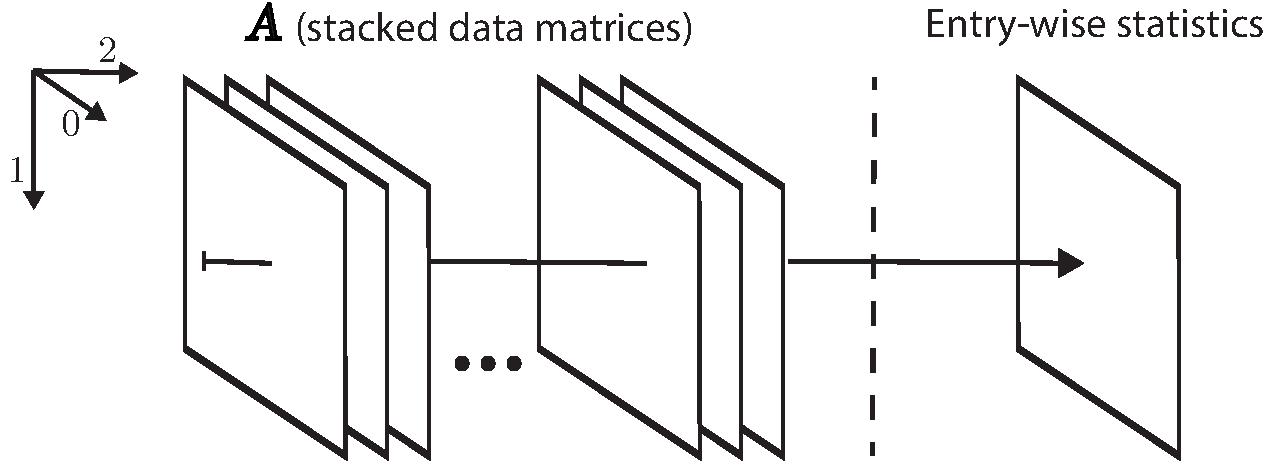
\includegraphics[width=0.6\textwidth]{figures/entryWiseStatistics}
	\caption{\label{fig:entryWiseStatistics}Illustration of how matrices are stacked to compute the entry-wise statistics $\sigma_{a,t}$, $\sigma_{a,t}^2$, $\tilde{A_{a,t}}$ and $\bar{A_{a,t}}$. See App. \ref{app:statisticsConsensusArchetypes} for values.}
\end{figure} 

\begin{figure}[h]
	\centering
	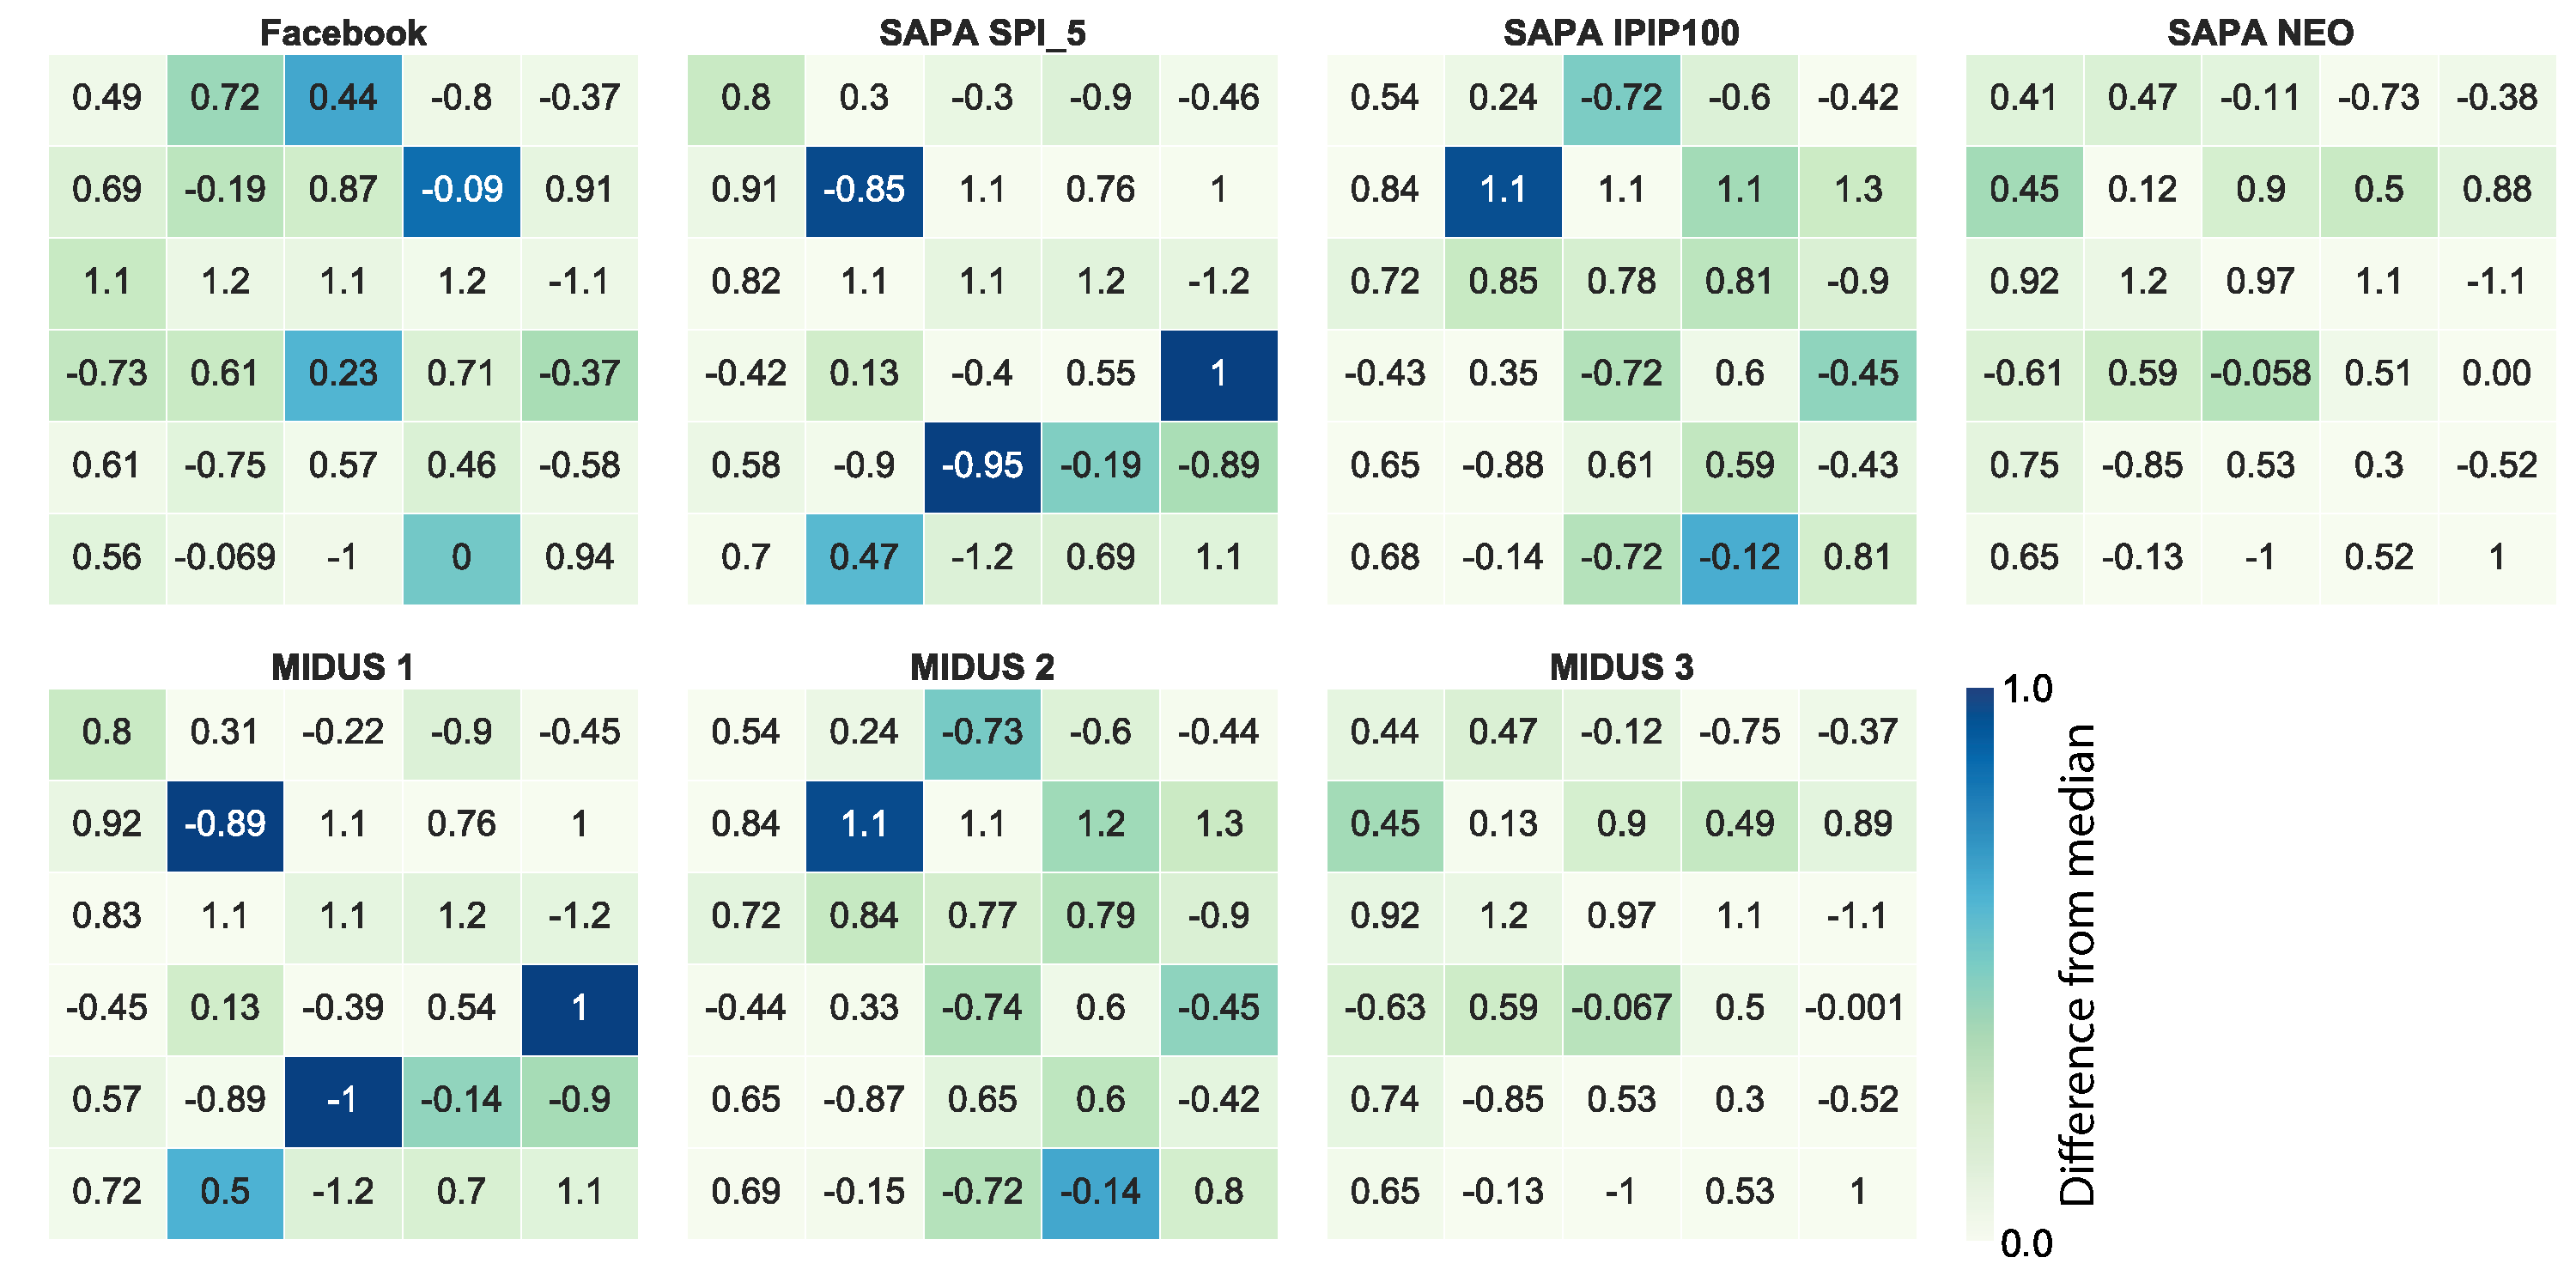
\includegraphics[width=\textwidth]{figures/medianDistances}
	\caption{\label{fig:medianDistances} Distances from archetype trait median in terms of archetype trait std. ($\sigma$-distance) for each dataset, visualized in color. Annotated values are rows of archetypes and BF trait values columns ordered by O, C, E, A and N. It is noted that the Sensible DTU dataset has many outliers compared to the other datasets.}
\end{figure}

First, to investigate which datasets should be used for computing CAs the following approach is taken. For each of the four datasets described in Sec. \ref{sec:datasets} six archetypes are computed such that every set of archetypes form a $d$-simplex ($d=5$) in its space, satisfying the ParTI principle described in Sec. \ref{subsubsec:paretoTaskInterence}. Rows in each matrix are sorted such that they correspond to the same archetypes across datasets\footnote{For spaces of larger dimensionality and more archetypes this should be done using K-Means with $d+1$ kernels, but since this is a small problem it is easier done manually.}. The matrices are stacked to produce a 3rd-order tensor, $\matr{A}$ and entry-wise median, $\tilde{A_{a,t}}$, and standard deviation values, $\sigma_{a,t}$, where $a$ and $t$ denote rows (archetypes) and columns (traits) respectively, are computed along the 2nd axis, as illustrated in Fig. \ref{fig:entryWiseStatistics} (see App. \ref{app:statisticsConsensusArchetypes} for these and more statistics). For each entry the distance from corresponding $\tilde{A_{a,t}}$ in terms of corresponding $\sigma_{a,t}$ is computed. This produces yields the matrices visualized in Fig. \ref{fig:medianDistances}}. The figure clearly shows the Sensible DTU dataset to be more rid with outliers compared to the others, the implications of which are discussed later. Because of this, it is decided to only use the three datasets \textit{Facebook}, \textit{SAPA} and \textit{MIDUS} for computing CAs.

\begin{figure}[h]
	\centering
	\begin{minipage}[l]{0.42\textwidth}
		\centering
		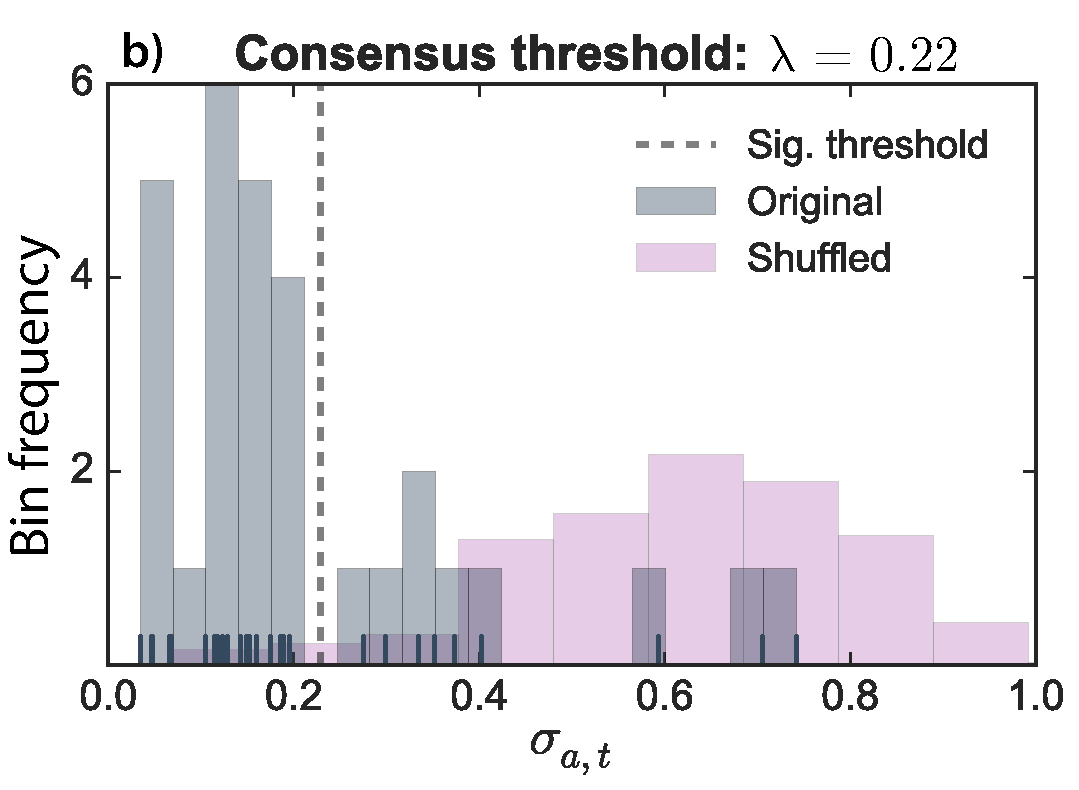
\includegraphics[width=\textwidth]{figures/varianceThreshold}
	\end{minipage}
	\begin{minipage}[r]{0.52\textwidth}
		\centering
		\vspace{-0.67cm}
		\includegraphics[width=\textwidth]{figures/consensusArchetypes}
	\end{minipage}
	\vspace{-0.25cm}
	\caption{\label{fig:varianceThreshold} \textbf{a)} Consensus threshold is chosen at 0.08, because it captures a natural seperation between high and low $\sigma_{a,t}^2$. \textbf{b)} CAs (rows). Mean archetypes where trait values, $\bar{A_{a,t}}$, are colored with respect to the consensus threshold: green signifies consensus and grey signifies above threshold non-consensus, i.e. undefined dimensions. Traits are named using the convention explained by Tab. \ref{tab:CANamingConvention}.}
\end{figure}

\begin{table}[h!]
	\centering
	\includegraphics[width=0.5\textwidth]{figures/CANamingConvention}
	\caption{\label{tab:CANamingConvention} CA naming convention. \^\, represents negative values and symbol size scales in discrete steps with absolute trait value.}
\end{table}

% \begin{figure}[h!]
% 	\centering
% 	\includegraphics[width=\textwidth]{figures/3darr}
% 	\caption{\label{fig:3darr}Archetypes in each dataset, where rows are sorted such that each figure-wide row holds points that correspond to the same consensus archetype. The bold values exemplify how $\sigma_t^2$ is computed across the datasets. $\sigma_t^2$ values are used to set a consensus threshold as shown in Fig. \ref{fig:varianceThreshold}.}
% \end{figure}

Across the three chosen datasets $\sigma_{a,t}^2$ are computed as illustrated in Fig. \ref{fig:entryWiseStatistics}. Fig. \ref{fig:varianceThreshold}.a shows a histogram/KDE plot of all $\sigma_{a,t}^2$, which reveals a natural seperation between low and high $\sigma_{a,t}^2$. Based on this a consensus threshold is chosen at 0.08 resulting in a consensus mask which is applied to the mean archetype trait values shown in Fig. \ref{fig:varianceThreshold}.b. Each CA is named after the convention shown in Tab. \ref{tab:CANamingConvention}

\subparagraph*{Discussion} The CAs found in the analysis can only be understood as personalities that belong to archetypes of \textit{real people}, and with this in mind many of them lend themselves to interpretation quite well. In the following each of the CAs are characterized using keywords from Fig. \ref{fig:bigfive} and the top of the authors head.

\begin{itemize}[label={},leftmargin=0cm]
\item $\,\,\,\,\,\,\,\,$\textbf{\achiever} \qquad Intelligent, wideOrderly, prepared and pays attention to detail (\textit{conscientious}), rarely sad and generally calm (non-\textit{neurotic}), but very unpleasant, insulting and feels little concern for others (non-\textit{agreeable}).
\item $\,\,\,\,\,\,\,\,\,\,\,\,$\textbf{\host} \qquad Talkative, sociable and adventurous (highly \textit{extroverted}), yet anxious, moody and often worried (highly \textit{neurotic}).
\item \textbf{\wildcard} \qquad Imaginative, intellectual and interested in abstractions (highly \textit{open}), orderly, prepared, pays attention to detail (highly \textit{conscientious}), talkative, sociable, adventurous (highly \textit{extroverted}), warm, sympathetic, interested in people (highly \textit{agreeable}) and rarely sad, generally calm, stable and confident (highly non-\textit{neurotic}).
\item $\,\,\,\,\,\,\,\,\,\,\,\,\,\,$\textbf{\loyalist} \qquad Not reflective, uninterested in abstractions and has poor imagination (highly non-\textit{open}), but orderly and prepared (\textit{conscientious}).
\item $\,\,\,\,\,\,\,\,\,\,\,\,\,$\textbf{\hippie} \qquad Imaginative and interested in abstractions (\textit{open}), very messy, careless and undependable (highly non-\textit{conscientious}), sociable and adventurous (\textit{extroverted}), and warm and interested in people (\textit{agreeable}).
\item $\,\,\,\,\,\,\,\,\,\,\,$\textbf{\follower} \qquad Very introverted, secretive, reclusive and silent (highly non-\textit{extroverted}).
\end{itemize}

It is interesting to observe how extremely confident the \wildcard CA is. 
Sensible DTU has more outliers because it is a narrower population and as such students to not occupy the full BF space normally occupied by broader western populations.
